\documentclass{article}
\usepackage[utf8]{inputenc}

%\usepackage{lmodern}
%\renewcommand*\familydefault{\sfdefault}

\usepackage{amsmath}
\usepackage{hyperref}
\usepackage{tikz}
\usetikzlibrary{matrix}
\usepackage{enumitem}
\setenumerate[0]{label=(\alph*)}
\usepackage{amsmath}
\usepackage{algorithm}
\usepackage[noend]{algpseudocode}

\makeatletter
\def\BState{\State\hskip-\ALG@thistlm}
\makeatother

\newcommand{\addend}{\text{\textsl{\color{gray}{Addend}}}}
\newcommand{\augend}{\text{\textsl{\color{gray}{Augend}}}}
\newcommand{\sumOut}{\text{\textsl{\color{gray}{Sum}}}}

\usepackage{array,mathtools}
\newcommand*{\carry}[1][1]{\overset{#1}}
\newcolumntype{B}[1]{r*{#1}{@{\,}r}}

% expandable loop (used to avoid scope problems in tabular cells with the
% standard \loop)
\def\boucle #1\repeat {#1\b@@cle {#1}\repeat \repeat }
\def\b@@cle #1{\repeat #1\b@@cle {#1}}

\makeatletter
\newcount\@nn
\newcount\@mm
\newcount\@base
\newcount\@baseminusone

% please do not use this at home
% #1 must be a counter name, not something expanding to a number.
\def\@arabalpha #1{\ifcase #10\or1\or2\or3\or4\or5\or6\or7\or8\or9\or 
A\or B\or C\or D\or E\or F\or G\or H\or I\or J\or K\or L\or M\or N\or O\or
P\or Q\or R\or S\or T\or U\or V\or W\or X\or Y\or Z\fi}

\newcommand{\baseexpansion}[2][2]{% no negative numbers please!
\def\@digits{}%
\@base#1\relax \@baseminusone\@base\advance\@baseminusone-1
\@nn #2\relax  % this is the number to be written in base #1
%
\ifnum\@baseminusone<36
\def\onerow{#1\kern.1em\hbox{\vrule
   \vtop {\hbox{\ \the\@nn}\kern.3ex\hrule height.1ex }} &%
   \global\@mm\@nn \global\divide\@mm\@base 
   \multiply\@mm\@base \advance\@nn-\@mm 
   \the\@nn \xdef\@digits{\@arabalpha\@nn\@digits}}%
\else
\def\onerow{#1\kern.1em\hbox{\vrule
   \vtop {\hbox{\ \the\@nn}\kern.3ex\hrule height.1ex }} &%
   \global\@mm\@nn \global\divide\@mm\@base 
   \multiply\@mm\@base \advance\@nn-\@mm 
   \the\@nn \xdef\@digits{\the\@nn.\@digits}}%
\fi
%
\leavevmode\oalign{$#2_{10}:$\hfil\cr
      $\left.
      \begin{tabular}{r|l}
         \boucle \onerow \\ \ifnum\@nn>\@baseminusone\global\@nn\@mm \repeat
      \end{tabular}\right\rbrace=
      \mathtt{\@digits}_{#1}$}}     % \hfil removed from the macro

\makeatother


\usepackage{xinttools}

\newcounter{bitindex}

\newcommand\bitpicture [3]{%
  \setlength{\unitlength}{0.85mm}
  \setlength{\fboxsep}{0mm}
  \begin{picture}(124,16)
    % sign bit
  \put(2,4){\framebox(4,8){#1}}
  % exponent
  \setcounter{bitindex}{1}%
  \xintFor* ##1 in {#2}
  \do
  {\put(\numexpr 2+4*\value{bitindex},4){\framebox(4,8){##1}}%
   \stepcounter{bitindex}}%
  % fraction
  \setcounter{bitindex}{1}%
  \xintFor* ##1 in {#3}
  \do
  {\put(\numexpr 34+4*\value{bitindex},4){\framebox(4,8){##1}}%
   \stepcounter{bitindex}}%
  % upper labels
  \put(0,14){\scriptsize{MSB}}
  \put(126,14){\scriptsize{LSB}}
  %lower labels
  \put(3,0){\scriptsize{S}}
  \put(7,0){\line(0,1){2}}
  \put(7,1){\vector(1,0){8}}
  \put(16,0){\scriptsize{Esponente}}
  \put(37,1){\vector(-1,0){8}}
  \put(37,0){\line(0,1){2}}
  \put(39,0){\line(0,1){2}}
  \put(39,1){\vector(1,0){38}}
  \put(79,0){\scriptsize{Mantissa}}
  \put(130,1){\vector(-1,0){38}}
  \put(130,0){\line(0,1){2}}
\end{picture}%
}

\title{Tutorato Architettura degli Elaboratori Modulo 1 (Lezione 2)}
\author{Francesco Pelosin }
\date{23 Ottobre 2019}

\begin{document}

\maketitle

\section{Numeri razionali in Base $b$}
\subsection{Virgola fissa}
Dato un numero razionale espresso con notazione a virgola fissa in Base $b$ su $n$ cifre intere e $m$ cifre razionali:

$$d_{n-1} d_{n-2} \dots d_{1} d_{0},d_{-1} d_{-2} \dots d_{m-1} d_{m}$$

\noindent Possiamo ricavare il suo corrispondente valore in decimale nel seguente modo:

$$d_{n-1}\cdot b^{n-1}+\dots +d_{1}\cdot b^{1}+d_{0}\cdot b^{0}+d_{-1}\cdot b^{-1}+\dots +d_{-m+1}\cdot b^{-m+1}+d_{-m}\cdot b^{-m}$$

\noindent Volendo trasformare un numero razionale espresso in Base 10 in una generica Base $b$ dobbiamo applicare il seguente procedimento:
\begin{itemize}
\item Trasformare la parte intera del numero da Base 10 a Base $b$ (applicando l'algoritmo visto nella precedente lezione).
\item Trasformare la parte frazionaria del numero in Base $b$. La trasformazione della parte frazionaria pu\`o essere computata procedendo per moltiplicazioni successive nel seguente modo:
\begin{itemize}
\item Moltiplichiamo la parte frazionaria del numero per $b$.
\item Continuiamo a moltiplicare il risultato ottenuto per $b$ tenendo presente che se il numero ottenuto \`e ha una parte intera maggiore di zero dobbiamo continuare con la sola parte frazionaria. La parte intera in ogni caso, diventa la nuova cifra frazionaria in base $b$
\item Andiamo avanti fino a quando la parte frazionaria diventa 0 oppure un risultato gi\`a ottenuto (periodicit\`a).
\end{itemize}
\end{itemize}

\subsubsection{Esercizi da Base 10 a Base $b$}

Convertire i seguenti numeri da Base 10 a Base $b$:
\begin{enumerate}
\item $310,63_{10} \rightarrow$ in Base 6
\item $321,225_{10} \rightarrow$ in Base 2
\item $519,51_{10} \rightarrow$ in Base 5
\item $921,75_{10} \rightarrow$ in Base 9
\end{enumerate}

\subsubsection{Soluzioni}
\begin{enumerate}
  \item Troviamo il valore in Base 6 della parte intera di $310,63_{10}$:
  $$\baseexpansion[6]{310}$$
  Troviamo il valore in Base 6 della parte frazionaria del numero procedendo per moltiplcazioni successive:
  \begin{center}
  \begin{tabular}{ l | c | r }
    & $\cdot$ 6&   \\
  0,63 & 3,78 & 3 \\
  0,78 & 4,68 & 4 \\
  \underline{0,68} & 4,08 & 4 \\  
  0,08 & 0,48 & 0 \\
  0,48 & 2,88 & 2 \\ 
  0,88 & 5,28 & 5 \\
  0,28 & 1,68 & 1 \\ 
  \underline{0,68} &  ... & ... \\ 
  \end{tabular}
  \end{center}
  

  Avendo trovato una ripetizione sappiamo che la parte frazionaria ha una periodicit\`a:
  
  $$0,63\textsubscript{10}=0,34\overline{40251}\textsubscript{6}$$

  Possiamo ora scrivere il corrispondente valore in base 6 del numero di partenza:

  $$310,63\textsubscript{10}=1234,34\overline{40251}\textsubscript{6}$$

  
  
  \item Troviamo il valore in Base 2 della parte intera di 321,225\textsubscript{10}:

  $$\baseexpansion{321}$$

  Troviamo il valore in Base 2 della parte frazionaria del numero procedendo per moltiplcazioni successive:
$$
 \begin{tabular}{ l | c | r }
    & $\cdot$ 2&   \\
  0,225 & 0,45 & 0 \\
  0,45  & 0,9  & 0 \\
  0,9   & 1,8  & 1 \\  
  \underline{0,8}   & 1,6  & 1 \\
  0,6   & 1,2  & 1 \\ 
  0,2   & 0,4  & 0 \\
  0,4   & 0,8  & 0 \\ 
  \underline{0,8}   & ...  & ... \\ 
  \end{tabular}
$$
  Avendo trovato una ripetizione sappiamo che la parte frazionaria avr\`a una periodicit\`a:

  $$0,225\textsubscript{10}=0,001\overline{1100}\textsubscript{2}$$

  Possiamo ora scrivere il corrispondente valore in Base 2 del numero di partenza:

  $$310,63\textsubscript{10}=101000001,001\overline{1100}\textsubscript{2}$$

  
  \item Troviamo il valore in base 5 della parte intera di 519,51\textsubscript{10}:
  $$\baseexpansion[5]{519}$$
  Troviamo il valore in base 5 della parte frazionaria del numero procedendo per moltiplcazioni successive:

  $$\begin{tabular}{ l | c | r }
    & $\cdot$ 5&   \\
  0,51 & 2,55 & 2 \\
  0,55 & 2,75 & 2 \\
  \underline{0,75} & 3,75 & 3 \\  
  \underline{0,75} & ...  & ... \\
  \end{tabular}
  $$
  Avendo trovato una ripetizione sappiamo che la parte frazionaria avr\`a una periodicit\`a:
$$0,51\textsubscript{10}=0,22\overline{3}\textsubscript{5}$$
  Possiamo ora scrivere il corrispondente valore in base 5 del numero di partenza:
$$519,51\textsubscript{10}=4034,22\overline{3}\textsubscript{2}$$

  \item Troviamo il valore in base 9 della parte intera di 921,75\textsubscript{10}:

  $$\baseexpansion[9]{921}\hfil$$

  Troviamo il valore in base 9 della parte frazionaria del numero procedendo per moltiplcazioni successive:
$$\begin{tabular}{ l | c | r }
    & $\cdot$ 9&   \\
  \underline{0,75} & 6,75 & 6 \\
  \underline{0,75} & ... & ... \\
  \end{tabular}
$$
  Avendo trovato una ripetizione sappiamo che la parte frazionaria avr\`a una periodicit\`a:
  $$0,75\textsubscript{10}=0,\overline{6}\textsubscript{9}$$
  Possiamo ora scrivere il corrispondente valore in base 5 del numero di partenza:
  $$921,75\textsubscript{10}=1233,\overline{6}\textsubscript{9}$$
  
\end{enumerate}

\subsubsection{Esercizi da Base $b$ a Base 10}
Tradurre i seguenti numeri in Base 10:
\begin{enumerate}
\item 11310,32\textsubscript{5}
\item 147,75\textsubscript{12}
\item 3A7,68\textsubscript{16}
\item 1703,12\textsubscript{8}
\end{enumerate}

\subsubsection{Soluzioni}
\begin{enumerate}
\item $11310,32_{5}=1\cdot 5^{4}+1\cdot 5^{3}+3\cdot 5^{2}+1\cdot 5^{1}+0\cdot 5^{0}+3\cdot 5^{-1}+2\cdot 5^{-2}=625+125+75+5+0,6+0,08=830,68_{10}$

\item $147,75_{12}=1\cdot 12^{2}+4\cdot 12^{1}+7\cdot 12^{0}+7\cdot 12^{-1}+5\cdot 12^{-2}=144+48+7+0,584+0,03473=199,61873_{10}$

\item $3A7,68_{16}=3\cdot 16^{2}+10\cdot 16^{1}+7\cdot 16^{0}+6\cdot 16^{-1}+8\cdot 16^{-2}=768+160+7+0,375+0,03125=935,40625_{10}$

\item $1703,12_{8}=1\cdot 8^{3}+7\cdot 8^{2}+0\cdot 8^{1}+3\cdot 8^{0}+1\cdot 8^{-1}+2\cdot 8^{-2}=512+448+3+0,125+0,03125=963,15625_{10}$
\end{enumerate}

\subsubsection{Esercizi da Base 10 a Base 2}
Convertire i seguenti numeri da Base 10 a Base 2:
\begin{enumerate}
\item 35,75\textsubscript{10}
\item 44,35\textsubscript{10}
\item 63,875\textsubscript{10}
\item 136,5625\textsubscript{10}
\item 192,625\textsubscript{10}
\item 255,90625\textsubscript{10}
\end{enumerate}

\subsubsection{Soluzioni}

\begin{enumerate}
  \item Troviamo il valore in Base 2 della parte intera di 35,75\textsubscript{10}:
  $$\baseexpansion{35}$$
  Troviamo il valore in base 6 della parte frazionaria del numero procedendo per moltiplcazioni successive:
  $$\begin{tabular}{ l | c | r }
    & $\cdot$ 2&   \\
  0,75 & 1,5 & 1 \\
  0,5  & \underline{1,0} & 1 \\
  0,0 &  &  \\  
  \end{tabular}$$
  Avendo ottenuto un risultato intero posso fermarmi e affermare che:
  $$0,75\textsubscript{10}=0,11\textsubscript{2}$$
  Possiamo ora scrivere il corrispondente valore in base 6 del numero di partenza:
  $$35,75\textsubscript{10}=100011,11\textsubscript{2}$$
  
  \item Troviamo il valore in Base 2 della parte intera di 44,35\textsubscript{10}:
  $$\baseexpansion{44}$$
  Troviamo il valore in Base 2 della parte frazionaria del numero procedendo per moltiplcazioni successive:
  $$\begin{tabular}{ l | c | r }
    & $\cdot$ 2&   \\
  0,35  & 0,7  & 0 \\
  0,7   & 1,4  & 1 \\
  \underline{0,4}   & 0,8  & 0 \\  
  0,8   & 1,6  & 1 \\
  0,6   & 1,2  & 1 \\ 
  0,2   & 0,4  & 0 \\
  \underline{0,4}   & 0,8  & 0 \\ 
  0,8   & ...  & ... \\ 
  \end{tabular}
$$
  Avendo trovato una ripetizione sappiamo che la parte frazionaria avr\`a una periodicit\`a:
  $$0,35\textsubscript{10}=0,01\overline{0110}\textsubscript{2}$$
  Possiamo ora scrivere il corrispondente valore in Base 2 del numero di partenza:
$$44,35\textsubscript{10}=101100,01\overline{0110}\textsubscript{2}$$
  
  \item Troviamo il valore in Base 2 della parte intera di 63,875\textsubscript{10}:
$$\baseexpansion{63}$$
  Troviamo il valore in Base 2 della parte frazionaria del numero procedendo per moltiplcazioni successive:
$$
\begin{tabular}{ l | c | r }
    & $\cdot$ 2&   \\
  0,875 & 1,75 & 1 \\
  0,75  & 1,5  & 1 \\
  0,5   & \underline{1,0}  & 1 \\  
  0,0   &  &  \\
  \end{tabular}
$$
  Avendo ottenuto un risultato intero posso fermarmi e affermare che:
$$0,875\textsubscript{10}=0,111\textsubscript{2}$$
  Possiamo ora scrivere il corrispondente valore in Base 2 del numero di partenza:
$$63,875\textsubscript{10}=111111,111\textsubscript{2}$$
  
  
  \item Troviamo il valore in Base 2 della parte intera di 136,5625\textsubscript{10}:
$$\baseexpansion{136}$$
  Troviamo il valore in Base 2 della parte frazionaria del numero procedendo per moltiplcazioni successive:
$$\begin{tabular}{ l | c | r }
    & $\cdot$ 2&   \\
  0,5625 & 1,125 & 1 \\
  0,125  & 0,25  & 0 \\
  0,25   & 0,5   & 0 \\  
  0,5    & \underline{1,0}   & 1  \\
  0,0    &   &  \\
  \end{tabular}
$$
  Avendo ottenuto un risultato intero posso fermarmi e affermare che:
$$0,5625\textsubscript{10}=0,1001\textsubscript{2}$$
  Possiamo ora scrivere il corrispondente valore in Base 2 del numero di partenza:
$$136,5625\textsubscript{10}=10001000,1001\textsubscript{2}$$
  
  \item Troviamo il valore in Base 2 della parte intera di 192,625\textsubscript{10}:
$$\baseexpansion{192}$$
  Troviamo il valore in Base 2 della parte frazionaria del numero procedendo per moltiplcazioni successive:
$$
\begin{tabular}{ l | c | r }
    & $\cdot$ 2&   \\
  0,625  & 1,25  & 1 \\
  0,25   & 0,5   & 0 \\
  0,5    & \underline{1,0}   & 1 \\  
  0,0    &   &  \\
  \end{tabular}
$$
  Avendo ottenuto un risultato intero posso fermarmi e affermare che:
$$0,625\textsubscript{10}=0,101\textsubscript{2}$$
  Possiamo ora scrivere il corrispondente valore in Base 2 del numero di partenza:
$$192,625\textsubscript{10}=11000000,101\textsubscript{2}$$
  
  \item Troviamo il valore in Base 2 della parte intera di 255,90625\textsubscript{10}:
$$\baseexpansion{255}$$
  Troviamo il valore in Base 2 della parte frazionaria del numero procedendo per moltiplcazioni successive:
$$\begin{tabular}{ l | c | r }
    & $\cdot$ 2&   \\
  0,90625  & 1,8125  & 1 \\
  0,8125   & 1,625   & 1 \\
  0,625    & 1,25    & 1 \\ 
  0,25     & 0,5     & 0 \\
  0,5      & \underline{1,0}  & 1 \\
  0,0    &   &  \\
  \end{tabular}
$$
  Avendo ottenuto un risultato intero posso fermarmi e affermare che:
$$0,90625\textsubscript{10}=0,11101\textsubscript{2}$$
  Possiamo ora scrivere il corrispondente valore in Base 2 del numero di partenza:
$$255,90625\textsubscript{10}=11111111,11101\textsubscript{2}$$
  
\end{enumerate}

\subsubsection{Esercizi da Base 2 a Base 10}
Tradurre i seguenti numeri in Base 10:
\begin{enumerate}
\item 100011,0111\textsubscript{2}
\item 101100,101\textsubscript{2}
\item 111111,0011\textsubscript{2}
\item 10001000,1111\textsubscript{2}
\item 11000000,11001\textsubscript{2}
\item 11111111,001\textsubscript{2}
\end{enumerate}

\subsubsection{Soluzioni}

\begin{enumerate}
\item $100011,0111_{2}=1\cdot 2^{5}+0\cdot 2^{4}+0\cdot 2^{3}+0\cdot 2^{2}+1\cdot 2^{1}+1\cdot 2^{0}+0\cdot 2^{-1}+1\cdot 2^{-2}+1\cdot 2^{-3}+1\cdot 2^{-4}=32+2+1+0,25+0,125+0,0625=35,4375_{10}$

\item $101100,101_{2}=1\cdot 2^{5}+0\cdot 2^{4}+1\cdot 2^{3}+1\cdot 2^{2}+0\cdot 2^{1}+0\cdot 2^{0}+1\cdot 2^{-1}+0\cdot 2^{-2}+1\cdot 2^{-3}=32+8+4+0,5+0,125=44,625_{10}$

\item $111111,0011_{2}=1\cdot 2^{5}+1\cdot 2^{4}+1\cdot 2^{3}+1\cdot 2^{2}+1\cdot 2^{1}+1\cdot 2^{0}+0\cdot 2^{-1}+0\cdot 2^{-2}+1\cdot 2^{-3}+1\cdot 2^{-4}=32+16+8+4+2+1+0,125+0,0625=63,1875_{10}$

\item $10001000,1111_{2}=1\cdot 2^{7}+0\cdot 2^{6}+0\cdot 2^{5}+0\cdot 2^{4}+1\cdot 2^{3}+0\cdot 2^{2}+0\cdot 2^{1}+0\cdot 2^{0}+1\cdot 2^{-1}+1\cdot 2^{-2}+1\cdot 2^{-3}+1\cdot 2^{-4}=128+8+0,5+0,25+0,125+0,0625=136,9375_{10}$

\item $11000000,11001_{2}=1\cdot 2^{7}+1\cdot 2^{6}+0\cdot 2^{5}+0\cdot 2^{4}+0\cdot 2^{3}+0\cdot 2^{2}+0\cdot 2^{1}+0\cdot 2^{0}+1\cdot 2^{-1}+1\cdot 2^{-2}+0\cdot 2^{-3}+0\cdot 2^{-4}+1\cdot 2^{-5}=128+64+0,5+0,25+0,03125=192,78125_{10}$

\item $11111111,001_{2}=1\cdot 2^{7}+1\cdot 2^{6}+1\cdot 2^{5}+1\cdot 2^{4}+1\cdot 2^{3}+1\cdot 2^{2}+1\cdot 2^{1}+1\cdot 2^{0}+0\cdot 2^{-1}+0\cdot 2^{-2}+1\cdot 2^{-3}=128+64+32+16+8+4+2+1+0,125=255,125_{10}$
\end{enumerate}

\subsection{Virgola mobile}
Nella notazione in virgola mobile (floating point) si usa la notazione scientifica normalizzata:

$$\pm 1,\underset{Mantissa}{\underbrace{mmmmmm}}\times 2^{\overset{Esponente}{\overbrace{eeee}}}$$

Su Base 2 i bit disponibili per la rappresentazione di un numero in virgola mobile, vengono suddivisi in:
\begin{itemize}
    \item Un bit per il segno $S$
    \item Un blocco di bit per l'esponente $E$
    \item Un blocco di bit per la mantissa $M$
\end{itemize}
In particolare, per la rappresentazione dei numeri in Base 2 in virgola mobile, si usa lo standard IEEE754, nello specifico:
\begin{itemize}
    \item IEEE754 a Singola Precisione (32 bit):
    \begin{itemize}
        \item 1 bit per il segno $S$
        \item 8 bit per l'esponente $E$
        \item 23 bit per la mantissa $M$
    \end{itemize}
    \item IEEE754 a Doppia Precisione (64 bit):
    \begin{itemize}
        \item 1 bit per il segno $S$
        \item 11 bit per l'esponente $E$
        \item 20+32 bit per la mantissa $M$
    \end{itemize}
     
\end{itemize}

Ricordiamo, che lo standard prevede la polarizzazione dell'esponente (per accelerare le operazioni di ordinamento):
\begin{itemize}
    \item IEEE754 a Singola Precisione (32 bit) $\rightarrow$ polarizziamo aggiungendo 127 all'esponente del numero
    \item IEEE754 a Doppia Precisione (64 bit) $\rightarrow$ polarizziamo aggiungendo 1023 ad all'esponente del numero
\end{itemize}
La presenza di un esponente polarizzato implica che il valore rappresentato da un numero in virgola mobile nella realtà sia dato da:

$$(-1)^{S} \times (1+Mantissa) \times 2^{E-127}$$

Ricordiamo, in oltre, che lo standard considera implicito il primo bit (sempre uguale a 1) dei numeri binari normalizzati.

\subsubsection{Esercizi}
Rappresentare i seguenti numeri in Base 2 secondo lo standard IEEE754 Singola Precisione (32 bit):
\begin{enumerate}
    \item 35,75\textsubscript{10}
    \item -63,875\textsubscript{10}
    \item 136,5625\textsubscript{10}
    \item -192,625\textsubscript{10}
\end{enumerate}

\subsubsection{Soluzioni}

\begin{enumerate}
    \item Essendo $35,75_{10}=100011,11_{2}$ riscriviamo il numero in notazione scientifica normalizzata Base 2:
$$+1,0001111\cdot2\textsuperscript{5}$$
    Identifichiamo segno esponente e mantissa:
    \begin{itemize}
        \item[] $S=0$
        \item[] $M=1+0,0001111=1,0001111$
        \item[] $E=5+127=132\textsubscript{10}=10000100\textsubscript{2}$
    \end{itemize}
    Ricordando che in singola precisione disponiamo di 32 bit rispettivamente 1 per il segno 8 per l'esponente e 23 per la  mantissa scriviamo:
    \begin{figure}[h!]
    \centering
    \bitpicture {0}{10000100}{00011110000000000000000}
    \end{figure} 
        
    \item Essendo $63,875_{10}=111111,111_{2}$ riscriviamo il numero in notazione scientifica normalizzata Base 2:
$$-1,11111111\cdot2\textsuperscript{5}$$
    Identifichiamo segno esponente e mantissa:
    \begin{itemize}
        \item[] $S=1$
        \item[] $M=1+0,11111111=1,11111111$
        \item[] $E=5+127=132\textsubscript{10}=10000100\textsubscript{2}$
    \end{itemize}
    Ricordando che in singola precisione disponiamo di 32 bit rispettivamente 1 per il segno 8 per l'esponente e 23 per la  mantissa scriviamo:
    \begin{figure}
    \centering
    \bitpicture {1}{10000100}{11111111000000000000000}
    \end{figure} 
    
    \item Essendo $136,5625_{10}=10001000,1001_{2}$ riscriviamo il numero in notazione scientifica normalizzata Base 2:
$$+1,00010001001\cdot 2\textsuperscript{7}$$
    Identifichiamo segno esponente e mantissa:
    \begin{itemize}
        \item[] $S=0$
        \item[] $M=1+0,00010001001=1,00010001001$
        \item[] $E=7+127=134\textsubscript{10}=10000110\textsubscript{2}$
    \end{itemize}
    Ricordando che in singola precisione disponiamo di 32 bit rispettivamente 1 per il segno 8 per l'esponente e 23 per la  mantissa scriviamo:
    \begin{figure}[h!]
    \centering
    \bitpicture {0}{10000110}{00010001001000000000000}
    \end{figure}
    
    \item Essendo $192,625_{10}=11000000,101_{2}$ riscriviamo il numero in notazione scientifica normalizzata Base 2:
$$-1,1000000101\cdot2\textsuperscript{7}$$
    Identifichiamo segno esponente e mantissa:
    \begin{itemize}
        \item[] $S=1$
        \item[] $M=1+0,1000000101=1,1000000101$
        \item[] $E=7+127=134\textsubscript{10}=10000110\textsubscript{2}$
    \end{itemize}
    Ricordando che in singola precisione disponiamo di 32 bit rispettivamente 1 per il segno 8 per l'esponente e 23 per la  mantissa scriviamo:
    \begin{figure}[h!]
    \centering
    \bitpicture {1}{10000110}{10000001010000000000000}
    \end{figure}
    
\end{enumerate}

\subsection{Somme di numeri Floating Point}

L'algoritmo per sommare numeri floating point (FP) espressi in Base 2 \`e il seguente:
\begin{enumerate}
    \item[1.] Confronto dell'esponente dei due numeri; scorrimento del numero più piccolo a destra finché il suo esponente non è uguale a quello del numero maggiore
    \item[2.] Somma dei significandi (nel caso sia una somma tra due numeri con segno diverso usare l'algoritmo di cambio di segno ed aggiungere un bit di segno per passare alla rappresentazione in complemento a due)
    \item[3.] Normalizzazione della somma, facendo scorrere la virgola verso sinistra e aumentando l'esponente, oppure farla scorrere verso destra e diminuendo l'esponente.
    \item[4.] Controllare se è avvenuto overflow o underflow dell'esponente. Nel caso positivo generare un'eccezione oppure, nel caso negativo, procedere con il prossimo step.
    \item[5.] Arrotondamento del significando al numero adeguato di bit.
    \item[6.] Controllare se il numero è normalizzato. In caso positivo terminare, in caso positivo tornare allo step 3.
\end{enumerate}
\subsubsection{Esercizi}
Considerando i numeri convertiti in floating point precedentemente:
\begin{itemize}
    \item[] A=35,75\textsubscript{10}
    \item[] B=-63,875\textsubscript{10}
    \item[] C=136,5625\textsubscript{10}
    \item[] D=-192,625\textsubscript{10}
\end{itemize}
Svolgere le seguenti somme ed esprimere il risultato secondo lo standard IEEE754 a Singola Precisione (32 bit):
\begin{enumerate}
    \item $A + B$
    \item $A + D$
    \item $B + C$
\end{enumerate}


\subsubsection{Soluzioni}
\begin{enumerate}
    \item La rappresentazione di $A$ nello standard IEEE754 Singola Precisione è:
        \begin{itemize}
            \item[] $S\textsubscript{A}=0$
            \item[] $M\textsubscript{A}=1+0,0001111=1,0001111$
            \item[] $E\textsubscript{A}=5+127=132\textsubscript{10}=10000100\textsubscript{2}$
        \end{itemize}

    La rappresentazione di $B$ nello standard IEEE754 Singola Precisione è:
    \begin{itemize}
        \item[] $S\textsubscript{B}=1$
        \item[] $M\textsubscript{B}=1+0,11111111=1,11111111$
        \item[] $E\textsubscript{B}=5+127=132\textsubscript{10}=10000100\textsubscript{2}$
    \end{itemize}
    Svolgiamo la somma A + B nel seguente modo:
    \begin{itemize}
        \item Allineamento degli esponenti: poiché gli esponenti sono uguali, non serve allinearli.
        \item Essendo $B$ un numero FP negativo (si guardi il bit di segno) usiamo l'algoritmo di cambio di segno ed esprimiamo i numeri in complemento a due:

$$M\textsubscript{A}=01,0001111$$
$$M\textsubscript{B}=01,11111111 \rightarrow 10,00000001$$
        \item Sommiamo:
        \begin{center}
        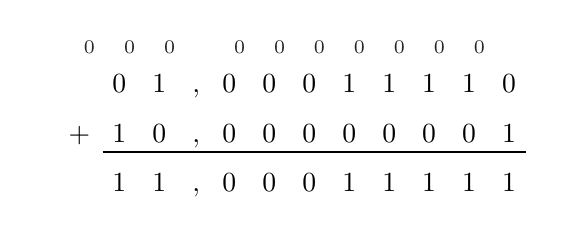
\begin{tikzpicture}[
            row 1/.style={font=\textsl,font=\scriptsize,black!85, anchor=west,
                inner sep=1.5pt},
            every node/.style={column sep=.5mm,row sep=1mm}]
            \matrix (m) [matrix of math nodes,
                nodes in empty cells,
                %nodes=draw
            ] 
            {
                & 0 & 0 & 0 &   & 0 & 0  & 0 & 0 & 0 & 0 & 0 &    &                  \\
                &   & 0 & 1 & , & 0 & 0  & 0 & 1 & 1 & 1 & 1 & 0  &[10mm]      \\
                & + & 1 & 0 & , & 0 & 0  & 0 & 0 & 0 & 0 & 0 & 1  &         \\ 
                &   & 1 & 1 & , & 0 & 0  & 0 & 1 & 1 & 1 & 1 & 1  &          \\                                                  
            };
        
            \draw[-,color=black,semithick] (m-3-3.south west) -- (m-3-13.south east);
        
        \end{tikzpicture}
        \label{binary_integer_addition}
        \end{center}
        Osserviamo che il bit di segno del risultato è 1. Utilizziamo l'algoritmo di cambio di segno per trovare il valore assoluto del numero:
$$M_{A}+M_{B}=11,00011111 \rightarrow 00,11100001$$
        Scriviamo il risutato della somma in notazione scientifica normalizzata Base 2:
$$A + B=-0,11100001\cdot 2^{5} = -1,1100001\cdot 2^{4}$$
    \end{itemize}
    Disponiamo ora di tutti i dati per rappresentare il risultato della somma secondo lo standard IEEE754 Singola Precisione:
    \begin{itemize}
        \item[] $S=1$
        \item[] $M=1+0,1100001=1,1100001$
        \item[] $E=4+127=131_{10}=10000011_{2}$
    \end{itemize}
    Ricordando che in singola precisione disponiamo di 32 bit rispettivamente 1 per il segno 8 per l'esponente e 23 per la  mantissa scriviamo:
    \begin{figure}[h!]
    \centering
    \bitpicture {1}{10000011}{11000010000000000000000}
    \end{figure}
    
    
    \item  La rappresentazione di $A$ nello standard IEEE754 Singola Precisione è:\begin{itemize}
            \item[] $S\textsubscript{A}=0$
            \item[] $M\textsubscript{A}=1+0,0001111=1,0001111$
            \item[] $E\textsubscript{A}=5+127=132\textsubscript{10}=10000100\textsubscript{2}$
        \end{itemize}
 La rappresentazione di $D$ nello standard IEEE754 Singola Precisione è:    \begin{itemize}
        \item[] $S\textsubscript{D}=1$
        \item[] $M\textsubscript{D}=1+0,1000000101=1,1000000101$
        \item[] $E\textsubscript{D}=7+127=134\textsubscript{10}=10000110\textsubscript{2}$
    \end{itemize}
    Svolgiamo la somma di $A+D$ nel seguente modo:
    \begin{itemize}
        \item Allineiamo l'esponente del numero pi\`u piccolo a quello del numero pi\`u grande (cio\`e allineiamo l'esponente di A):
$$A=1,0001111\cdot2\textsuperscript{5}=0,010001111\cdot2\textsuperscript{7}$$
        \item Essendo $D$ un numero FP negativo (si guardi il bit di segno) usiamo l'algoritmo di cambio di segno ed esprimiamo i numeri in complemento a due:
            \begin{itemize}
                \item[] $M\textsubscript{A}=00,010001111$
                \item[] $M\textsubscript{D}=01,1000000101 \rightarrow 10,0111111011$
            \end{itemize}
        \item Sommiamo:
        \begin{center}
        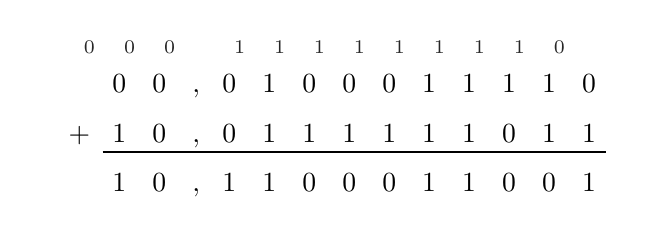
\begin{tikzpicture}[
            row 1/.style={font=\textsl,font=\scriptsize,black!85, anchor=west,
                inner sep=1.5pt},
            every node/.style={column sep=.5mm,row sep=1mm}]
            \matrix (m) [matrix of math nodes,
                nodes in empty cells,
                %nodes=draw
            ] 
            {
                & 0& 0 & 0 &   & 1 & 1  & 1  & 1 & 1 & 1 & 1 & 1 & 0  &   &  \\
                &  & 0 & 0 & , & 0 & 1  & 0 & 0 & 0 & 1 & 1 & 1 & 1  & 0 &[10mm]      \\
                & +& 1 & 0 & , & 0 & 1  & 1 & 1 & 1 & 1 & 1 & 0 & 1  & 1 &  \\ 
                &  & 1 & 0 & , & 1 & 1  & 0 & 0 & 0 & 1 & 1 & 0 & 0  & 1 &  \\                                                  
            };
        
            \draw[-,color=black,semithick] (m-3-3.south west) -- (m-3-15.south east);
        
        \end{tikzpicture}
        \label{binary_integer_addition}
        \end{center}
        Per prima cosa osserviamo che il bit del segno del risultato \`e 1. Utilizziamo l'algoritmo di cambio di segno per trovare il valore assoluto del numero:
$$M\textsubscript{A}+M\textsubscript{D}=10,1100011001 \rightarrow 01,0011100111$$
        Scriviamo il risultato della somma in notazione scientifica normalizzata Base2:
$$ A + D=-1,0011100111\cdot2\textsuperscript{7}$$
    \end{itemize}
    Disponiamo ora di tutti i dati per rappresentare il risultato della somma secondo lo standard IEEE754 Singola Precisione:
    \begin{itemize}
        \item[] $S=1$
        \item[] $M=1+0,0011100111=1,0011100111$
        \item[] $E=7+127=134\textsubscript{10}=10000110\textsubscript{2}$
    \end{itemize}
    Ricordando che in singola precisione disponiamo di 32 bit rispettivamente 1 per il segno 8 per l'esponente e 23 per la  mantissa scriviamo:
    \begin{figure}[h!]
    \centering
    \bitpicture {1}{10000110}{00111001110000000000000}
    \end{figure}


    \item La rappresentazione di $B$ nello standard IEEE754 Singola Precisione è:
    \begin{itemize}
        \item[] $S\textsubscript{B}=1$
        \item[] $M\textsubscript{B}=1+0,11111111=1,11111111$
        \item[] $E\textsubscript{B}=5+127=132\textsubscript{10}=10000100\textsubscript{2}$
    \end{itemize}
    La rappresentazione di $C$ nello standard IEEE754 Singola Precisione è:
    \begin{itemize}
        \item[] $S\textsubscript{C}=0$
        \item[] $M\textsubscript{C}=1+0,00010001001=1,00010001001$
        \item[] $E\textsubscript{C}=7+127=134\textsubscript{10}=10000110\textsubscript{2}$
    \end{itemize}
    Svolgiamo la somma B + C nel seguente modo:
    \begin{itemize}
        \item Allineiamo l'esponente del numero pi\`u piccolo a quello del numero pi\`u grande (cio\`e allineiamo l'esponente di B):
$$B=-1,11111111\cdot2\textsuperscript{5}=-0,0111111111\cdot2\textsuperscript{7}$$
        \item Essendo B un numero FP negativo (si guardi il bit di segno) usiamo l'algoritmo di cambio di segno ed esprimiamo i numeri in complemento a due:
            \begin{itemize}
                \item[] $M\textsubscript{B}=00,0111111111 \rightarrow 11,1000000001$
                \item[] $M\textsubscript{C}=01,00010001001$
            \end{itemize}
        \item Ora possiamo sommare le due mantisse:
        \begin{center}
        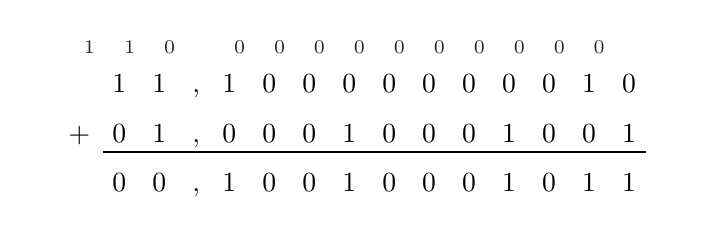
\begin{tikzpicture}[
            row 1/.style={font=\textsl,font=\scriptsize,black!85, anchor=west,
                inner sep=1.5pt},
            every node/.style={column sep=.5mm,row sep=1mm}]
            \matrix (m) [matrix of math nodes,
                nodes in empty cells,
                %nodes=draw
            ] 
            {
                & 1 & 1 & 0 &   & 0 & 0 & 0 & 0 & 0 & 0 & 0 & 0 & 0 & 0 &   & \\
                &   & 1 & 1 & , & 1 & 0 & 0 & 0 & 0 & 0 & 0 & 0 & 0 & 1 & 0 &[10mm] \\
                & + & 0 & 1 & , & 0 & 0 & 0 & 1 & 0 & 0 & 0 & 1 & 0 & 0 & 1 &  \\ 
                &   & 0 & 0 & , & 1 & 0 & 0 & 1 & 0 & 0 & 0 & 1 & 0 & 1 & 1 &  \\                                                  
            };
        
            \draw[-,color=black,semithick] (m-3-3.south west) -- (m-3-16.south east);
        
        \end{tikzpicture}
        \label{binary_integer_addition}
        \end{center}
        Per prima cosa osserviamo che il bit del segno del risultato \`e 0. Scriviamo il risultato della somma in notazione scientifica normalizzata Base2:
$$B + C=+0,10010001011\cdot2\textsuperscript{7}=+1,0010001011\cdot2\textsuperscript{6}$$
    \end{itemize}
    Disponiamo ora di tutti i dati per rappresentare il risultato della somma secondo lo standard IEEE754:
    \begin{itemize}
        \item[] $S=0$
        \item[] $M=1+0,0010001011=1,0010001011$
        \item[] $E=6+127=133\textsubscript{10}=10000101\textsubscript{2}$
    \end{itemize}
    Ricordando che in singola precisione disponiamo di 32 bit rispettivamente 1 per il segno 8 per l'esponente e 23 per la  mantissa scriviamo:
    \begin{figure}[h!]
    \centering
    \bitpicture {0}{10000101}{00100010110000000000000}
    \end{figure}
\end{enumerate}

\subsubsection{Esercizi}
Date le seguenti sequenze binarie espresse su 32 bit:
\begin{itemize}
    \item[] $A = 01111011100110101111000000000000$
    \item[] $B = 11111010011010100100000000000000$
    \item[] $C = 01111100010100101111100000000000$
    \item[] $D = 11111010100011011100000000000000$
\end{itemize}
Interpretarli come numeri FP espressi secondo lo standard IEEE754 Sine svolgere le seguenti operazioni:
\begin{enumerate}
    \item $A - B$
    \item $B + C$
    \item $C - B$
    \item $D + B$
\end{enumerate}

\subsubsection{Soluzioni}
\begin{itemize}
    \item Riscriviamo $A$ come:
    \begin{figure}[h!]
    \centering
    \bitpicture {0}{11110111}{00110101111000000000000}
    \end{figure}
    \\Identifichiamo segno esponente e mantissa::
    \begin{itemize}
        \item[] $S\textsubscript{A}=0$
        \item[] $M\textsubscript{A}=1+0,00110101111=1,00110101111$
        \item[] $E\textsubscript{A}=11110111\textsubscript{2}=247\textsubscript{10}=120+127$
    \end{itemize}
    Infine esprimiamo $A$ in notazione scientifica normalizzata Base 2:
    $$A=+1,00110101111\cdot2\textsuperscript{120}$$
    
    \item Riscriviamo $B$ come:
    \begin{figure}[h!]
    \centering
    \bitpicture {1}{11110100}{11010100100000000000000}
    \end{figure}
    \\Identifichiamo segno esponente e mantissa::
    \begin{itemize}
        \item[] $S\textsubscript{B}=1$
        \item[] $M\textsubscript{B}=1+0,110101001=1,110101001$
        \item[] $E\textsubscript{B}=11110100\textsubscript{2}=244\textsubscript{10}=117+127$
    \end{itemize}
    Infine esprimiamo $B$ in notazione scientifica normalizzata Base 2:
$$ B=-1,110101001\cdot2\textsuperscript{117}$$
    
    \item Riscriviamo $C$ come:
    \begin{figure}[h!]
    \centering
    \bitpicture {0}{11111000}{10100101111100000000000}
    \end{figure}
    \\Identifichiamo segno esponente e mantissa::
    \begin{itemize}
        \item[] $S\textsubscript{C}=0$
        \item[] $M\textsubscript{C}=1+0,101001011111=1,101001011111$
        \item[] $E\textsubscript{C}=11111000\textsubscript{2}=248\textsubscript{10}=121+127$
    \end{itemize}
    Infine esprimiamo $C$ in notazione scientifica normalizzata Base 2:
$$C=+1,101001011111\cdot2\textsuperscript{121}$$

    \item Riscriviamo $D$ come:
    \begin{figure}[h!]
    \centering
    \bitpicture {1}{11110101}{00011011100000000000000}
    \end{figure}
    \\Identifichiamo segno esponente e mantissa::
    \begin{itemize}
        \item[] $S\textsubscript{D}=1$
        \item[] $M\textsubscript{D}=1+0,000110111=1,000110111$
        \item[] $E\textsubscript{D}=11110101\textsubscript{2}=245\textsubscript{10}=118+127$
    \end{itemize}
    Infine esprimiamo $D$ in notazione scientifica normalizzata Base 2:
$$D=-1,000110111\cdot2\textsuperscript{118}$$
    
\end{itemize}
Ora svolgiamo le operazioni:
\begin{enumerate}
    \item La rappresentazione di $A$ nello standard IEEE754 Singola Precisione è:
    \begin{itemize}
        \item[] $S\textsubscript{A}=0$
        \item[] $M\textsubscript{A}=1+0,00110101111=1,00110101111$
        \item[] $E\textsubscript{A}=11110111\textsubscript{2}=247\textsubscript{10}=120+127$
    \end{itemize}
    La rappresentazione di $B$ nello standard IEEE754 Singola Precisione è:
    \begin{itemize}
        \item[] $S\textsubscript{B}=1$
        \item[] $M\textsubscript{B}=1+0,110101001=1,110101001$
        \item[] $E\textsubscript{B}=11110100\textsubscript{2}=244\textsubscript{10}=117+127$
    \end{itemize}
    Sapendo che B \`e un numero negativo possiamo riscrivere la sottrazione come segue $A +(-B)$. Cambiamo dunque il bit di segno di $B$ e procediamo con l'algoritmo di somma:
    \begin{itemize}
        \item Allineiamo l'esponente del numero pi\`u piccolo a quello del numero pi\`u grande (cio\`e allineiamo l'esponente di B):
$$B=+1,110101001\cdot2\textsuperscript{117}=+0,001110101001\cdot2\textsuperscript{120}$$
        \item Essendo entrambi i numeri positivi possiamo direttamente fare la somma:
$$M\textsubscript{A}=+1,00110101111$$
$$M\textsubscript{B'}=+0,001110101001$$
       Eseguiamo la somma:
        \begin{center}
        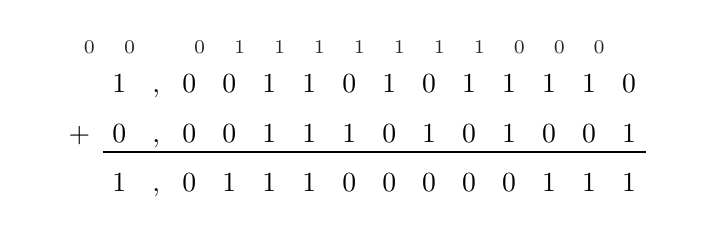
\begin{tikzpicture}[
            row 1/.style={font=\textsl,font=\scriptsize,black!85, anchor=west,
                inner sep=1.5pt},
            every node/.style={column sep=.5mm,row sep=1mm}]
            \matrix (m) [matrix of math nodes,
                nodes in empty cells,
                %nodes=draw
            ] 
            {
                  & 0 & 0 &   & 0 & 1 & 1 & 1 & 1 & 1 & 1 & 1 & 0 & 0 & 0 & & \\
                & & 1 & , & 0 & 0 & 1 & 1 & 0 & 1 & 0 & 1 & 1 & 1 & 1 & 0 & [10mm]      \\
                &+& 0 & , & 0 & 0 & 1 & 1 & 1 & 0 & 1 & 0 & 1 & 0 & 0 & 1 &  \\ 
                & & 1 & , & 0 & 1 & 1 & 1 & 0 & 0 & 0 & 0 & 0 & 1 & 1 & 1 &  \\                                                  
            };
        
            \draw[-,color=black,semithick] (m-3-3.south west) -- (m-3-16.south east);
        
        \end{tikzpicture}
        \label{binary_integer_addition}
        \end{center}
        Avendo sommato due numeri positivi il risultato \`e sicuramente positivo quindi possiamo scrivere:
$$M\textsubscript{A}+M\textsubscript{B}=+1,011100000111$$
        Riscriviamo il risultato in notazione scientifica normalizzata Base 2 (osserviamo che la rappresentazione è già normalizzata):
$$A + B=+1,011100000111 \cdot 2\textsuperscript{120}$$
    \end{itemize}
    Disponiamo ora di tutti i dati per rappresentare il risultato della somma secondo lo standard IEEE754 Singola Precisione:
    \begin{itemize}
        \item[] $S=0$
        \item[] $M=1+0,011100000111=1,011100000111$
        \item[] $E=120+127=247\textsubscript{10}=11110111\textsubscript{2}$
    \end{itemize}
    Ricordando che in singola precisione disponiamo di 32 bit rispettivamente 1 per il segno 8 per l'esponente e 23 per la  mantissa scriviamo:
    \begin{figure}[h!]
    \centering
    \bitpicture {0}{11110111}{01110000011100000000000}
    \end{figure}
    

    
    \item La rappresentazione di $B$ nello standard IEEE754 Singola Precisione è:
    \begin{itemize}
        \item[] $S\textsubscript{B}=1$
        \item[] $M\textsubscript{B}=1+0,110101001=1,110101001$
        \item[] $E\textsubscript{B}=11110100\textsubscript{2}=244\textsubscript{10}=117+127$
    \end{itemize}
    La rappresentazione di $C$ nello standard IEEE754 Singola Precisione è::
    \begin{itemize}
        \item[] $S\textsubscript{C}=0$
        \item[] $M\textsubscript{C}=1+0,101001011111=1,101001011111$
        \item[] $E\textsubscript{C}=11111000\textsubscript{2}=248\textsubscript{10}=121+127$
    \end{itemize}
        Svolgiamo la somma B + C nel seguente modo:
    \begin{itemize}
        \item Allineiamo l'esponente del numero pi\`u piccolo a quello del numero pi\`u grande (cio\`e allineiamo l'esponente di B):
        $$B=-1,110101001\cdot 2\textsuperscript{117}=-0,0001110101001\cdot 2\textsuperscript{121}$$
        \item Essendo B un numero FP negativo (si guardi il bit di segno) usiamo l'algoritmo di cambio di segno ed esprimiamo i numero in complemento a due:

$$M\textsubscript{B}=00,0001110101001 \rightarrow 11,1110001010111$$
$$M\textsubscript{C}=01,101001011111$$

        \item Eseguiamo la somma:
        \begin{center}
        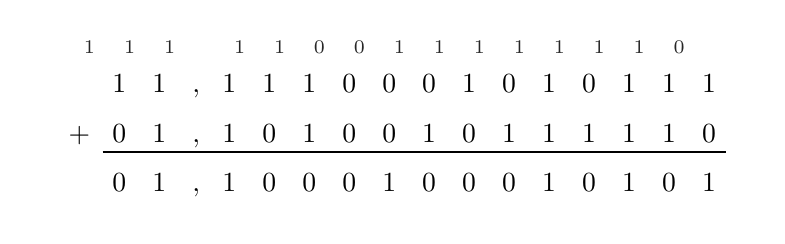
\begin{tikzpicture}[
            row 1/.style={font=\textsl,font=\scriptsize,black!85, anchor=west,
                inner sep=1.5pt},
            every node/.style={column sep=.5mm,row sep=1mm}]
            \matrix (m) [matrix of math nodes,
                nodes in empty cells,
                %nodes=draw
            ] 
            {
                & 1 & 1 & 1 &   & 1 & 1 & 0 & 0 & 1 & 1 & 1 & 1 & 1 & 1 & 1 & 0 &   & \\
                &   & 1 & 1 & , & 1 & 1 & 1 & 0 & 0 & 0 & 1 & 0 & 1 & 0 & 1 & 1 & 1 &[10mm] \\
                & + & 0 & 1 & , & 1 & 0 & 1 & 0 & 0 & 1 & 0 & 1 & 1 & 1 & 1 & 1 & 0 &  \\ 
                &  & 0 & 1 & , & 1 & 0 & 0 & 0 & 1 & 0 & 0 & 0 & 1 & 0 & 1 & 0 & 1 &  \\                                                  
            };
        
            \draw[-,color=black,semithick] (m-3-3.south west) -- (m-3-18.south east);
        
        \end{tikzpicture}
        \label{binary_integer_addition}
        \end{center}
        Osserviamo che il bit del segno del risultato \`e 0. Possiamo ora scrivere il risutato della somma secondo la notazione scientifica normalizzata in Base 2 (osserviamo che la rappresentazione è già normalizzata):
$$B + C=+1,1000100010101\cdot 2\textsuperscript{121}$$
    \end{itemize}
    Disponiamo ora di tutti i dati per rappresentare il risultato della somma secondo lo standard IEEE754 Singola Precisione:
    \begin{itemize}
        \item[] $S=0$
        \item[] $M=1+0,1000100010101=1,1000100010101$
        \item[] $E=121+127=248_{10}=11111000_{2}$
    \end{itemize}
    Ricordando che in singola precisione disponiamo di 32 bit rispettivamente 1 per il segno 8 per l'esponente e 23 per la  mantissa scriviamo:
    \begin{figure}[h!]
    \centering
    \bitpicture {0}{11111000}{10001000101010000000000}
    \end{figure}
    
    
    \item La rappresentazione di $C$ nello standard IEEE754 Singola Precisione è:
    \begin{itemize}
        \item[] $S_{C}=0$
        \item[] $M_{C}=1+0,101001011111=1,101001011111$
        \item[] $E_{C}=11111000_{2}=248_{10}=121+127$
    \end{itemize}
    La rappresentazione di $B$ nello standard IEEE754 Singola Precisione è::
    \begin{itemize}
        \item[] $S_{B}=1$
        \item[] $M_{B}=1+0,110101001=1,110101001$
        \item[] $E_{B}=11110100_{2}=244_{10}=117+127$
    \end{itemize}
    Sapendo che B \`e un numero negativo possiamo riscrivere la sottrazione come segue $C +(-B)$. Cambiamo dunque il bit di segno di $B$ e procediamo con l'algoritmo di somma:
    \begin{itemize}
        \item Allineiamo l'esponente del numero pi\`u piccolo a quello del numero pi\`u grande (cio\`e allineiamo l'esponente di $B$):
$$B=+1,110101001\cdot2\textsuperscript{117}=+0,0001110101001\cdot2\textsuperscript{121}$$
        \item Essendo entrambi i numeri positivi possiamo direttamente fare la somma:

$$M\textsubscript{C}=1,101001011111$$
$$M\textsubscript{B}=0,0001110101001$$
       Eseguiamo la somma come segue:
        \begin{center}
        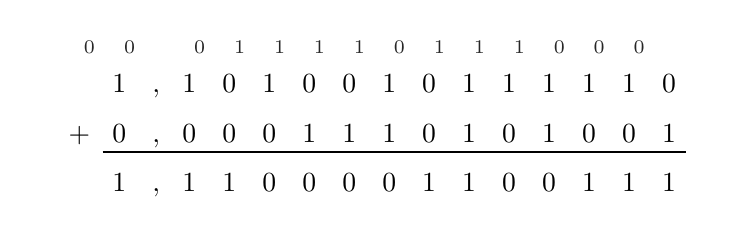
\begin{tikzpicture}[
            row 1/.style={font=\textsl,font=\scriptsize,black!85, anchor=west,
                inner sep=1.5pt},
            every node/.style={column sep=.5mm,row sep=1mm}]
            \matrix (m) [matrix of math nodes,
                nodes in empty cells,
                %nodes=draw
            ] 
            {
                & 0 & 0 &  & 0 & 1 & 1 & 1 & 1 & 0 & 1 & 1 & 1 & 0 & 0 & 0 &  &  \\
                & & 1 & , & 1 & 0 & 1 & 0 & 0 & 1 & 0 & 1 & 1 & 1 & 1 & 1 & 0 & [10mm]      \\
                &+& 0 & , & 0 & 0 & 0 & 1 & 1 & 1 & 0 & 1 & 0 & 1 & 0 & 0 & 1 &  \\ 
                & & 1 & , & 1 & 1 & 0 & 0 & 0 & 0 & 1 & 1 & 0 & 0 & 1 & 1 & 1 &\\                                                  
            };
        
            \draw[-,color=black,semithick] (m-3-3.south west) -- (m-3-17.south east);
        
        \end{tikzpicture}
        \label{binary_integer_addition}
        \end{center}
        Avendo sommato due numeri positivi il risultato \`e sicuramente positivo quindi possiamo scrivere:
$$M_{C}+M_{B}=1,1100001100111$$
        Scriviamo il risutato della somma secondo la notazione scientifica normalizzata in Base 2 (osserviamo che la rappresentazione è già normalizzata):
$$C + B=+1,1100001100111\cdot2\textsuperscript{121}$$
    \end{itemize}
    Disponiamo ora di tutti i dati per rappresentare il risultato della somma secondo lo standard IEEE754 Precisione Singola:
    \begin{itemize}
        \item[] $S=0$
        \item[] $M=1+0,1100001100111=1,1100001100111$
        \item[] $E=121+127=248_{10}=11111000_{2}$
    \end{itemize}
    Ricordando che in singola precisione disponiamo di 32 bit rispettivamente 1 per il segno 8 per l'esponente e 23 per la  mantissa scriviamo:
    \begin{figure}[h!]
    \centering
    \bitpicture {0}{11111000}{11000011001110000000000}
    \end{figure}

    \newpage
    
    \item La rappresentazione di $D$ nello standard IEEE754 Singola Precisione è:
    \begin{itemize}
        \item[] $S_{D}=1$
        \item[] $M_{D}=1+0,000110111=1,000110111$
        \item[] $E_{D}=11110101_{2}=245_{10}=118+127$
    \end{itemize}
    La rappresentazione di $B$ nello standard IEEE754 Singola Precisione è::
    \begin{itemize}
        \item[] $S_{B}=1$
        \item[] $M_{B}=1+0,110101001=1,110101001$
        \item[] $E_{B}=11110100_{2}=244_{10}=117+127$
    \end{itemize}
    Svolgiamo la somma D + B nel seguente modo:
    \begin{itemize}
        \item Allineiamo l'esponente del numero pi\`u piccolo a quello del numero pi\`u grande (cio\`e allineiamo l'esponente di B):
$$B=-1,110101001\cdot2\textsuperscript{117}=-0,1110101001\cdot2\textsuperscript{118}$$
        \item Essendo $D$ e $B$ numeri FP negativi (si guardi il bit di segno) possiamo sommare il loro valore assoluto tenendoci a mente che il risultato sarà sicuramente negativo. Procediamo dunque con la somma:
        \begin{center}
        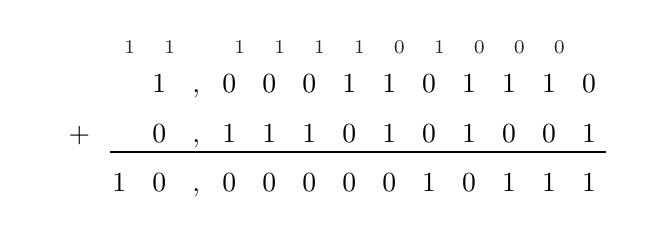
\begin{tikzpicture}[
            row 1/.style={font=\textsl,font=\scriptsize,black!85, anchor=west,
                inner sep=1.5pt},
            every node/.style={column sep=.5mm,row sep=1mm}]
            \matrix (m) [matrix of math nodes,
                nodes in empty cells,
                %nodes=draw
            ] 
            {
                  & & 1 & 1 &   & 1 & 1 & 1 & 1 & 0 & 1 & 0 & 0 & 0 & & \\
                & & & 1 & , & 0 & 0 & 0 & 1 & 1 & 0 & 1 & 1 & 1 & 0 & [10mm]      \\
                &+& & 0 & , & 1 & 1 & 1 & 0 & 1 & 0 & 1 & 0 & 0 & 1 &  \\ 
                && 1 & 0 & , & 0 & 0 & 0 & 0 & 0 & 1 & 0 & 1 & 1 & 1 &\\                                               
            };
        
            \draw[-,color=black,semithick] (m-3-3.south west) -- (m-3-15.south east);
        
        \end{tikzpicture}
        \label{binary_integer_addition}
        \end{center}
        \textbf{N.B:} è importante non interpretare l'uno nella posizione più significativa come il segno del risultato. Questo perchè stiamo sommando valori assoluti.
        
        Notiamo che è necessario eseguire la normalizzazione per rappresentare il risultato in notazione scientifica normalizzata Base 2:
$$D + B=-10,0000010111\cdot2\textsuperscript{118}=-1,00000010111\cdot2\textsuperscript{119}$$
    \end{itemize}
    Disponiamo ora di tutti i dati per rappresentare il risultato della somma secondo lo standard IEEE754 Precisione Singola:
    \begin{itemize}
        \item[] $S=1$
        \item[] $M=1+0,00000010111=1,00000010111$
        \item[] $E=119+127=246_{10}=11110110_{2}$
    \end{itemize}
    Ora ricordando che in singola precisione disponiamo di 32 bit rispettivamente 1 per il segno 8 per l'esponente e 23 per la  mantissa scriviamo:
    \begin{figure}[h!]
    \centering
    \bitpicture {0}{11110110}{00000010111000000000000}
    \end{figure}    
    
\end{enumerate}

\section{Risorse Esterne}

\begin{itemize}
    \item Floating Point Numbers - Computerphile \\ \href{https://www.youtube.com/watch?v=PZRI1IfStY0}{https://www.youtube.com/watch?v=PZRI1IfStY0} 
\end{itemize}



\end{document}





